\iffalse
\let\negmedspace\undefined
\let\negthickspace\undefined
\documentclass[journal,12pt,twocolumn]{IEEEtran}
\usepackage{cite}
\usepackage{amsmath,amssymb,amsfonts,amsthm}
\usepackage{algorithmic}
\usepackage{graphicx}
\usepackage{textcomp}
\usepackage{xcolor}
\usepackage{txfonts}
\usepackage{listings}
\usepackage{enumitem}
\usepackage{mathtools}
\usepackage{gensymb}
\usepackage{comment}
\usepackage[breaklinks=true]{hyperref}
\usepackage{tkz-euclide}
\usepackage{listings}
\usepackage{gvv}
\def\inputGnumericTable{}
\usepackage[latin1]{inputenc}
\usepackage{color}
\usepackage{array}
\usepackage{longtable}
\usepackage{calc}
\usepackage{multirow}
\usepackage{hhline}
\usepackage{ifthen}
\usepackage{lscape}

\newtheorem{theorem}{Theorem}[section]
\newtheorem{problem}{Problem}
\newtheorem{proposition}{Proposition}[section]
\newtheorem{lemma}{Lemma}[section]
\newtheorem{corollary}[theorem]{Corollary}
\newtheorem{example}{Example}[section]
\newtheorem{definition}[problem]{Definition}
\newcommand{\BEQA}{\begin{eqnarray}}
\newcommand{\EEQA}{\end{eqnarray}}
\newcommand{\define}{\stackrel{\triangle}{=}}
\theoremstyle{remark}
\newtheorem{rem}{Remark}
\begin{document}

\bibliographystyle{IEEEtran}
\vspace{3cm}

\title{GATE 2022  -AE 63}
\author{EE23BTECH11057 - Shakunaveti Sai Sri Ram Varun$^{}$% &lt;-this % stops a space
}
\maketitle
\newpage
\bigskip
\vspace{2cm}
\textbf{Question: }
The time delay between the peaks of the voltage signals $ v_1\brak{t}= \cos\brak{{6t+60\degree}}$ and $ v_2\brak{t} = -\sin\brak{{6t}}$ is \rule{1cm}{0.15mm}s
\begin{enumerate}
    \item[(A)] $ \frac{300\pi}{360}$
    \item[(B)]$ \frac{10\pi}{360}$
    \item[(C)] $ \frac{50\pi}{360}$
    \item[(D)] $ \frac{200\pi}{360}$  
\end{enumerate}
\hfill(GATE BM 2022 QUESTION 18)\\
\textbf{Solution}:\\
\fi
\begin{table}[h!] 
\centering
\begin{tabular}{|c|c|c|}
    \hline
    \textbf{Parameter} & \textbf{Description} & \textbf{Value} \\
    \hline
    $v_1\brak{t}$ & Input voltage signal 1 & $ \cos\brak{{6t+60\degree}}$\\
    \hline
    $v_2\brak{t}$ & Input voltage signal 2 &$ -\sin\brak{{6t}}$ \\
    \hline
    $\Delta \phi$ & Phase difference between two input signals & ? \\
    \hline
    $\Delta t$ & Time difference between maxima of two input signals & ? \\
    \hline
    $\omega$ & angular frequency of input voltages& $ 6$\\
    \hline
\end{tabular}





\caption{input values}
\label{tab: Table2022bm18}
\end{table}
From the values given in the \tabref{tab: Table2022bm18}:
\begin{align}
v_1\brak{t} &= \cos\brak{{6t+60\degree}}\\ \label{eq: 2022bm181}
v_2\brak{t} &= -\sin{\brak{6t}}\\
\implies v_2\brak{t} &= \cos{\brak{6t + 90\degree}} \label{eq: 2022bm182}
\end{align}
From \eqref{eq: 2022bm181} and \eqref{eq: 2022bm182},
phase difference between two voltage signals is $ 30\degree$.
From formula,
\begin{align}
    \Delta \phi &= \frac{\Delta t}{\frac{2\pi}{\omega}}360\\
    \therefore \Delta t &= \frac{10\pi}{360}s
\end{align}
Hence, option B is correct.
\begin{figure}[h!]
    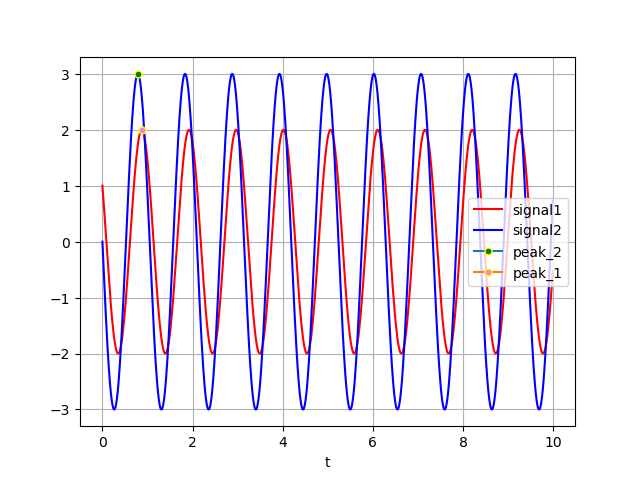
\includegraphics[width = 0.8\columnwidth]{2022/BM/18/figs/Figure_1.png}
    \caption{Figure of input voltage signals}
    \centering
    \label{fig: bm_18_2022}
\end{figure}

